%%%%%%%%%%%%%%%%%%%%%%%%%%%%%%%%%%%%%%%%%%%%%%%%%%%%%%%%%%%%%%%%%%%%%%%%%%%%%%%%
%2345678901234567890123456789012345678901234567890123456789012345678901234567890
%        1         2         3         4         5         6         7         8

\documentclass[letterpaper, 12 pt, conference]{ieeeconf}  % Comment this line out
                                                          % if you need a4paper
%\documentclass[a4paper, 10pt, conference]{ieeeconf}      % Use this line for a4
                                                          % paper

\IEEEoverridecommandlockouts                              % This command is only
                                                          % needed if you want to
                                                          % use the \thanks command
\overrideIEEEmargins
% See the \addtolength command later in the file to balance the column lengths
% on the last page of the document



% The following packages can be found on http:\\www.ctan.org
\usepackage{graphicx} % for pdf, bitmapped graphics files
\usepackage{graphics}
%\usepackage{epsfig} % for postscript graphics files
%\usepackage{mathptmx} % assumes new font selection scheme installed
%\usepackage{times} % assumes new font selection scheme installed
\usepackage{amsmath} % assumes amsmath package installed
\usepackage{amssymb}  % assumes amsmath package installed
\usepackage{hyperref}
\usepackage{bm}
\usepackage{algorithm2e}

\newcommand{\by}{\textbf{y}}
\newcommand{\bx}{\textbf{x}}
\newcommand{\bX}{\textbf{X}}
\newcommand{\bK}{\textbf{K}}
\newcommand{\cov}{\text{cov}}

\title{\LARGE \bf
Gaussian Processes for Crime Prediction
}

%\author{ \parbox{3 in}{\centering Luis Perez*
%         \thanks{*Use the $\backslash$thanks command to put information here}\\
%         Faculty of Electrical Engineering, Mathematics and Computer Science\\
%         University of Twente\\
%         7500 AE Enschede, The Netherlands\\
%         {\tt\small h.kwakernaak@autsubmit.com}}
%         \hspace*{ 0.5 in}
%         \parbox{3 in}{ \centering Alex Wang**
%         \thanks{**The footnote marks may be inserted manually}\\
%        Department of Electrical Engineering \\
%         Wright State University\\
%         Dayton, OH 45435, USA\\
%         {\tt\small pmisra@cs.wright.edu}}
%}

\author{Luis Perez$^{1}$ and Alex Wang$^{2}$% <-this % stops a space
\thanks{*A project for CS281, Fall 2015, Harvard University}% <-this % stops a space
\thanks{$^{1}$luisperez@college.harvard.edu}%
\thanks{$^{2}$alexwang@college.harvard.edu}%
}


\begin{document}



\maketitle
\thispagestyle{empty}
\pagestyle{empty}


%%%%%%%%%%%%%%%%%%%%%%%%%%%%%%%%%%%%%%%%%%%%%%%%%%%%%%%%%%%%%%%%%%%%%%%%%%%%%%%%
\begin{abstract}

Gaussian processes are a powerful Bayesian non-parametric model for machine learning that, unlike parametric models, can learn the underlying functions themselves. They have been successful when applied to a variety of tasks, such as inferring CO2 levels or detecting human motion. In this paper, we consider the problem of predicting future crime in a geographic area. Though average crime rates in the United States have been in the decline for the last few years, it is still useful to many groups, such as law enforcement, city officials, home buyers, etc., to be able to predict where and when crime will occur. Using recent data from various cities around the U.S., we explore how Gaussian processes under a variety of different kernels might help with this regression task. We compare these models to current baseline approaches which consists of taking the average over time or using linear regression along with other approaches.

\end{abstract}


%%%%%%%%%%%%%%%%%%%%%%%%%%%%%%%%%%%%%%%%%%%%%%%%%%%%%%%%%%%%%%%%%%%%%%%%%%%%%%%%
\section{INTRODUCTION}

- what the paper is about
- what problem it solves
- why the problem is interesting
- what's new in this paper

\section{MODEL}

Formally, a Gaussian process (GP) is a collection of random variables, any finite number of which have a joint Gaussian distribution \cite{c1}. A more intuitive understanding of a GP is as a distribution over functions. Then in training a GP, we attempt to learn the underlying function, as seen in \ref{gm}. If a function $f(\bx)$ follows a GP distribution, then we write
$$f(\bx) \sim GP(m(\bx), \kappa(\bx, \bx'))$$
where the GP completely specified by a mean function $m(x)$ and positive definite covariance function $\kappa(\bx, \bx')$, which are defined to be
$$m(x) = \mathbb{E}[f(x)]$$
$$\kappa(x, x') = \mathbb{E}[(f(\bx) - m(\bx))(f(\bx') - m(\bx'))]$$

Following the definition of a GP, given a collection of points \bX, $f(\bX)$ follows a multivariate normal distribution:
$$p(\textbf{f}|\bX) = \mathcal{N}(\textbf{f}|\bm{\mu}, \bK)$$
$$K_{ij} = \kappa(\bx_i, \bx_j)$$
$$\mu = (m(\bx_1), \dots, m(\bx_N))$$

The biggest decision in using Gaussian processes is the choice of the kernel function. The predictive performance of the GP is almost exclusively determined by the kernel function. The reason the kernel function is so important is that the kernel function determines if two points are similar, and if so, then the function value at those points are similar \cite{c2}. Thus, the kernel function determines the overall shape that the GP will try to learn.

A common choice for the kernel function is the squared exponential function. We present the multivariate form:
$$k_{\text{SE}}(\bx, \bx') = \sigma_f^2 \exp(-\frac{1}{2}(\bx - \bx')^\top \textbf{M} (\bx - \bx'))$$
where \textbf{M} is a diagonal matrix: $\textbf{M} = \text{diag}(\textbf{l}^-2)$. The parameters are $\sigma_f^2$, the vertical scale of the function, and $\textbf{l}$, the horizontal scale with $l_d$ the scale factor for dimension $d$. A large scale factor for a dimension means that the feature is relatively less important. Often times we also assume that we have noisy output, so we add the noise term $\sigma_\epsilon^2 \delta_{\bx\bx'}$ with $\delta_{\bx\bx'} = 1$ if $\bx = \bx'$, $0$ otherwise.

Two other kernels worth mentioning because we make use of them in this paper are the periodic kernel:
$$k_{\text{per}}(\bx, \bx') = \sigma_f^2 \exp(-\frac{1}{2} \sum_d (\frac{\sin(\frac{\pi}{\lambda} (x_d - x'_d))}{l})^2$$
As the name suggests, the periodic kernel is periodic, and thus is useful for capturing cyclic patterns in data. The parameters $\sigma_f^2$ again controls the vertical and horizontal scales respectively, while $\lambda$ controls the wavelength along dimension $d$.

We also have the linear kernel:
$$k_{\text{lin}}(\bx, \bx') = \sigma_b^2 + \sigma_f^2(\bx - \textbf{c})^\top(\bx' - \textbf{c})$$
The parameters $\sigma_b^2$ and $\sigma_v^2$ are the bias and scale term, similar to that of linear regression. In fact, if we were to simply use the linear kernel as our covariance function, we would actually be performing Bayesian linear regression \cite{c3}. The reason we include this kernel is that we can combine kernels via simple operations such as addition or multiplication and still have a valid kernel. Combining kernels in this way allows us to more accurately model different types of patterns.

   \begin{figure}[thpb]
      \centering
      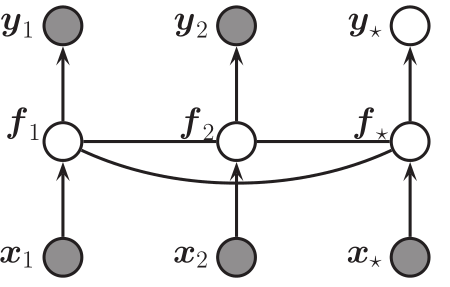
\includegraphics[scale=1.0]{graphical_model.PNG}
      %\framebox{\parbox{3in}{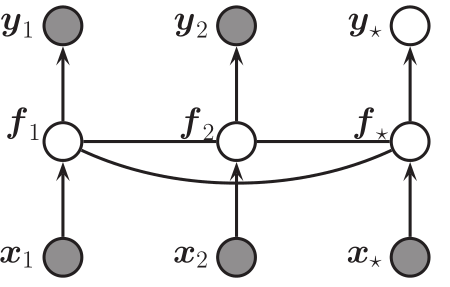
\includegraphics[scale=1.0]{graphical_model.PNG}}}
      \caption{Mixed graphical model for a noisy Gaussian process with two training points and one test point $\bx^*$. The function values $f_i = f(\bx_i)$ are all interconnected with edge weight $\kappa(\bx_i, \bx_j)$ while $y_i$ is the noisy output. We want to be able to predict $f(\bx^*)$. Figure borrowed from \cite{c2}}
      \label{gm}
   \end{figure}

\section{INFERENCE}

We now describe how to make predictions with Gaussian process regression. We assume we have seen data points $\{\bx_i, y_i\}_{i=1}^N$ where $y_i$ is the noisy output of the underlying function $f$. In other words, $y_i = f(\bx_i) + \epsilon$ with $\epsilon \sim \mathcal{N}(0, \sigma_\epsilon^2)$. We denote $\bX = \{\bx_i\}_{i=1}^N$ and $\by = \{y_i\}_{i=1}^N$. We want to make predictions on a new set of inputs $\bX^* = \{\textbf{x}^*_i\}_{i=1}^M$. Equivalently, we want $f(\textbf{x}^*_i)$ for all $i$, the entire vector of which we denote $\textbf{f}^*$.

From our model, we know that $\textbf{f}$ and $\textbf{f}^*$ is jointly Gaussian distributed:
$$\begin{pmatrix}
\by \\ \textbf{f}^*
\end{pmatrix} \sim \mathcal{N}\begin{pmatrix}
\textbf{0}, \begin{pmatrix}
\bK_y & \bK_* \\
\bK_*^\top & \bK_{**}
\end{pmatrix}
\end{pmatrix}
$$
where we assume that the mean of both is zero, $\bK_* = \cov(\by, \textbf{f}^*)$, and $\bK_{**} = \cov(\textbf{f}^*, \textbf{f}^*)$. Then we can use standard Gaussian conjugacy results to get the condition distribution of $\textbf{f}^*$:
$$p(\textbf{f}^*|\bX^*,\bX, \by) = \mathcal{N}(\textbf{f}^*|\bm{\mu}_*, \bm{\Sigma}_*)$$
$$\bm{\mu}_* = \bK_*^\top \bK_y^{-1} \by$$
$$\bm{\Sigma}_* = \bK_{**} - \bK_*^\top \bK_y^{-1} \bK_*$$
We take for our predictions the maximum a posteriori estimate, which for a Gaussian is the mean.

One complication is that it is not numerically stable to simply invert $\bK_y$ to compute the mean. Instead, we use a Cholesky decomposition, which we know exists because the kernel is positive definite. So, the final algorithm, which we take from Murphy \cite{c2}, is as follows
% \RestyleAlgo{boxed}
\RestyleAlgo{boxruled}
\LinesNumbered
\begin{algorithm}[ht]
  \caption{GP Regression\label{alg}}
  \textbf{L} = cholesky($\bK_y$) \\
  $\bm{\alpha} = \textbf{L}^\top \backslash (\textbf{L} \backslash \by))$ \\
  $\bm{\mu_*} = \bK_*^\top\bm{\alpha} $ \\
  $\log p(\by | \bX) = -\frac{1}{2}\by^\top \bm{\alpha} - \sum_i \log L_{ii} - \frac{N}{2}\log(2\pi)$
\end{algorithm}

\section{RELATED WORK}

Though the data-driven techniques for crime prediction have received increase research focus in recent years, there has been surprisingly little research on applying machine learning techniques to the task of crime prediction. Traditionally, most research has focused on either identifying hotspots of crime or clustering criminal activity by type of crime. Our paper falls in the former, and we proceed as such.

The simplest approach to crime hotspotting, and indeed one used often in practice, is simply to analyze historical data and take historical high crime areas to be the high crime areas in the future \cite{c6}. The current state of the art in However, most attention has gone towards identifying spatial patterns in crime data. Temporal patterns in the data receive far less attention \cite{c5}.

- talk about
\begin{enumerate}
\item previous applications of GPs to time series, spatial data
\item previous attempts to predict crime
- a lot of focus on hot spot mapping + clustering; not a lot of attempts at prediction
\end{enumerate}

\section{EXPERIMENTAL SETUP}

\subsection{Dataset}

We use public city crime datasets from Boston, San Francisco, and Chicago. These datasets document reported crimes that occur from 2012-2015, 2003-2015, and 2001-2015 respectively. Each dataset contains information on the type of crime, the time and date of the crime, geographic information including ward and latitude/longitude, and more. For our experiments, we extract

We bucket the data
Split the data
\subsection{Baselines}



\subsection{Implementation}

We implemented Gaussian process regression ourselves as well as two kernels, the squared exponential kernel and a periodic kernel. To verify the correctness of our code, we compare the computed likelihood of our model against that of the Gpy library for the same kernel and inputs (\url{https://github.com/SheffieldML/GPy}).

\section{RESULTS}

Figures to include:
\begin{enumerate}
\item marginal likelihood vs N
\item marginal likelihoods for different optimized kernels (fixed N)
\item predicted heat maps vs true
\end{enumerate}

\subsection{Figures and Tables}

We keep this around so we know how to position figures. Positioning Figures and Tables: Place figures and tables at the top and bottom of columns. Avoid placing them in the middle of columns. Large figures and tables may span across both columns. Figure captions should be below the figures; table heads should appear above the tables. Insert figures and tables after they are cited in the text. Use the abbreviation ÒFig. 1Ó, even at the beginning of a sentence.

\begin{table}[h]
\caption{An Example of a Table}
\label{table_example}
\begin{center}
\begin{tabular}{|c||c|}
\hline
One & Two\\
\hline
Three & Four\\
\hline
\end{tabular}
\end{center}
\end{table}


   \begin{figure}[thpb]
      \centering
      \framebox{\parbox{3in}{We suggest that you use a text box to insert a graphic (which is ideally a 300 dpi TIFF or EPS file, with all fonts embedded) because, in an document, this method is somewhat more stable than directly inserting a picture.
}}
      %\includegraphics[scale=1.0]{figurefile}
      \caption{Inductance of oscillation winding on amorphous
       magnetic core versus DC bias magnetic field}
      \label{figurelabel}
   \end{figure}

\section{CONCLUSIONS}

We add a conclusion that describes what we did, as well as future work / steps to take
- incorporate additional data, a number of paper use Twitter

\addtolength{\textheight}{-12cm}   % This command serves to balance the column lengths
                                  % on the last page of the document manually. It shortens
                                  % the textheight of the last page by a suitable amount.
                                  % This command does not take effect until the next page
                                  % so it should come on the page before the last. Make
                                  % sure that you do not shorten the textheight too much.

%%%%%%%%%%%%%%%%%%%%%%%%%%%%%%%%%%%%%%%%%%%%%%%%%%%%%%%%%%%%%%%%%%%%%%%%%%%%%%%%



%%%%%%%%%%%%%%%%%%%%%%%%%%%%%%%%%%%%%%%%%%%%%%%%%%%%%%%%%%%%%%%%%%%%%%%%%%%%%%%%



%%%%%%%%%%%%%%%%%%%%%%%%%%%%%%%%%%%%%%%%%%%%%%%%%%%%%%%%%%%%%%%%%%%%%%%%%%%%%%%%

\section*{ACKNOWLEDGMENT}

We may have an acknowledgment section where we thank the course staff.



%%%%%%%%%%%%%%%%%%%%%%%%%%%%%%%%%%%%%%%%%%%%%%%%%%%%%%%%%%%%%%%%%%%%%%%%%%%%%%%%

References are important to the reader; therefore, each citation must be complete and correct. If at all possible, references should be commonly available publications.



\begin{thebibliography}{99}

\bibitem{c1} Rasmussen, Carl Edward, and Christopher K. I. Williams. "Regression." Gaussian Processes for Machine Learning. Cambridge: MIT, 2006. Online.
\bibitem{c2} Murphy, Kevin P. "Gaussian Processes." Machine Learning a Probabilistic Perspective. Cambridge, Mass.: MIT, 2012. Print.
\bibitem{c3} Duvenaud, David. Automatic model construction with Gaussian processes. Diss. University of Cambridge, 2014.
\bibitem{c4} Chainey, Spencer, Lisa Tompson, and Sebastian Uhlig. "The utility of hotspot mapping for predicting spatial patterns of crime." Security Journal 21.1 (2008): 4-28.
\bibitem{c5} Ratcliffe, Jerry H. "The hotspot matrix: A framework for the spatio‐temporal targeting of crime reduction." Police practice and research 5.1 (2004): 5-23.
\bibitem{c6} Perry, Walt L. Predictive policing: The role of crime forecasting in law enforcement operations. Rand Corporation, 2013.

\end{thebibliography}




\end{document}
